\chapter{Stream Browser}
\label{streambrowser}

\section{Introduction}

The stream browser is the primary navigation pane for quick access to instrument settings and channels. By default in a
new ngscopeclient session it is docked to the left side of the window but it can be repositioned as needed.

\begin{figure}[H]
\centering
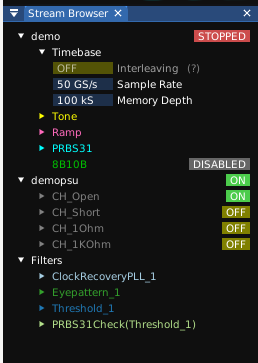
\includegraphics[width=7cm]{ng-images/streambrowser.png}
\caption{Example configuration of the stream browser}
\label{streambrowser}
\end{figure}

NOTE: The stream browser is one of the more recent additions to ngscopeclient and is undergoing rapid development. Some
changes to appearance and interaction metaphors should be expected in upcoming versions as we unify the user interface
to be more consistent for all types of instrument.

\section{Filters}

The "filters" node contains a list of all filter graph blocks active in the current session. Expanding the node for a
given filter will show a list of output streams.

\section{Instruments}

The node for each instrument contains a list of all channels on the instrument, whether enabled or not. Depending on
the type of instrument, additional nodes with commonly used settings such as timebase configuration may be available.

Color coded ``badges" are displayed in the right margin next to channels or instruments in some cases, displaying
context-dependent information such as trigger state, power supply or signal generator on/off status, etc. These badges
are clickable to change the relevant setting.

\section{Adding streams}

Instrument channels, filters, and streams can be dragged from the browser to other parts of ngscopeclient in order to
visualize or interact with data from them. For example:

\begin{itemize}
\item Drag a scalar stream to the measurements window to display its real-time value
\item Drag a currently-inactive channel to the filter graph view to add a node for the channel so it can be used
\item Drag a stream to a waveform area to display it in that plot
\end{itemize}
